\chapter{圖}

無向圖的節點定義如下:
\begin{Code}
// 無向圖的節點
struct UndirectedGraphNode {
    int label;
    vector<UndirectedGraphNode *> neighbors;
    UndirectedGraphNode(int x) : label(x) {};
};
\end{Code}


\section{Clone Graph} %%%%%%%%%%%%%%%%%%%%%%%%%%%%%%
\label{sec:clone-graph}


\subsubsection{描述}
Clone an undirected graph. Each node in the graph contains a \code{label} and a list of its \code{neighbours}.


OJ's undirected graph serialization:
Nodes are labeled uniquely.

We use \code{\#} as a separator for each node, and \code{,} as a separator for node label and each neighbour of the node.
As an example, consider the serialized graph \code{\{0,1,2\#1,2\#2,2\}}.

The graph has a total of three nodes, and therefore contains three parts as separated by \code{\#}.
\begin{enumerate}
\item First node is labeled as 0. Connect node 0 to both nodes 1 and 2.
\item Second node is labeled as 1. Connect node 1 to node 2.
\item Third node is labeled as 2. Connect node 2 to node 2 (itself), thus forming a self-cycle.
\end{enumerate}

Visually, the graph looks like the following:
\begin{Code}
       1
      / \
     /   \
    0 --- 2
         / \
         \_/
\end{Code}


\subsubsection{分析}
廣度優先遍歷或深度優先遍歷都可以。


\subsubsection{DFS}
\begin{Code}
// LeetCode, Clone Graph
// DFS,時間複雜度O(n),空間複雜度O(n)
class Solution {
public:
    UndirectedGraphNode *cloneGraph(const UndirectedGraphNode *node) {
        if(node == nullptr) return nullptr;
        // key is original node,value is copied node
        unordered_map<const UndirectedGraphNode *,
                            UndirectedGraphNode *> copied;
        clone(node, copied);
        return copied[node];
    }
private:
    // DFS
    static UndirectedGraphNode* clone(const UndirectedGraphNode *node,
            unordered_map<const UndirectedGraphNode *,
            UndirectedGraphNode *> &copied) {
        // a copy already exists
        if (copied.find(node) != copied.end()) return copied[node];

        UndirectedGraphNode *new_node = new UndirectedGraphNode(node->label);
        copied[node] = new_node;
        for (auto nbr : node->neighbors)
            new_node->neighbors.push_back(clone(nbr, copied));
        return new_node;
    }
};
\end{Code}


\subsubsection{BFS}
\begin{Code}
// LeetCode, Clone Graph
// BFS,時間複雜度O(n),空間複雜度O(n)
class Solution {
public:
    UndirectedGraphNode *cloneGraph(const UndirectedGraphNode *node) {
        if (node == nullptr) return nullptr;
        // key is original node,value is copied node
        unordered_map<const UndirectedGraphNode *,
                            UndirectedGraphNode *> copied;
        // each node in queue is already copied itself
        // but neighbors are not copied yet
        queue<const UndirectedGraphNode *> q;
        q.push(node);
        copied[node] = new UndirectedGraphNode(node->label);
        while (!q.empty()) {
            const UndirectedGraphNode *cur = q.front();
            q.pop();
            for (auto nbr : cur->neighbors) {
                // a copy already exists
                if (copied.find(nbr) != copied.end()) {
                    copied[cur]->neighbors.push_back(copied[nbr]);
                } else {
                    UndirectedGraphNode *new_node =
                            new UndirectedGraphNode(nbr->label);
                    copied[nbr] = new_node;
                    copied[cur]->neighbors.push_back(new_node);
                    q.push(nbr);
                }
            }
        }
        return copied[node];
    }
};
\end{Code}


\subsubsection{相關題目}
\begindot
\item 無
\myenddot

\section{Network Delay Time} %%%%%%%%%%%%%%%%%%%%%%%%%%%%%%
\label{sec:network-delay-time}


\subsubsection{描述}
There are N network nodes, labelled 1 to N.

Given times, a list of travel times as directed edges times[i] = (u, v, w), where u is the source node, v is the target node, and w is the time it takes for a signal to travel from source to target.

Now, we send a signal from a certain node K. How long will it take for all nodes to receive the signal? If it is impossible, return -1.

\begin{center}
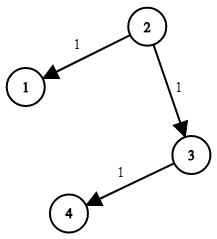
\includegraphics[width=100pt]{network-delay-time.png}\\
\figcaption{Rotate Image}\label{fig:network-delay-time}
\end{center}

\begin{Code}
Input: times = [[2,1,1],[2,3,1],[3,4,1]], N = 4, K = 2
Output: 2
\end{Code}

\begin{enumerate}
\item N will be in the range [l, 100]
\item K will be in the range [l, N]
\item The length of times will be in the range [l, 6000].
\item All edges times[i] = (u, v, w) will have l <= u, v <= N and 0 <= w <= 100.
\end{enumerate}
\subsubsection{分析}
廣度優先遍歷
Use Djikstra Algorithm. Find a minium path from one source to one end.


\subsubsection{Djikstra}
\begin{Code}
// LeetCode, Clone Graph
// DFS,時間複雜度O(ELogV),空間複雜度O(V^2)
class Solution {
public:
int networkDelayTime(vector<vector<int>>& times, int endPoint, int startPoint)
    {
        // key: startNode value: neighbours
        unordered_map<int, list<GraphNode> > graph = BuildGraph(times);
        // fail when start point cannot be reached
        if (graph.find(startPoint) == graph.end()) return -1;
        
        // PrintGraph(graph);
        vector<int> distCache(endPoint, INT_MAX); distCache[startPoint - 1] = 0;
        set<pair<int, int> > queue; // pair first: node number, pair second: cost

        queue.insert(make_pair(startPoint, 0));
        while (!queue.empty())
        {
            pair<int, int> curNode = *queue.begin();
            queue.erase(queue.begin());

            if (curNode.first == endPoint) break; // When endPoint find

            const auto& it = graph.find(curNode.first);
            if (it == graph.end()) continue; // skip if no neighbour
            for (const GraphNode& neighbour : it->second)
            {
                int curDist = distCache[curNode.first - 1] + neighbour.m_weight;
                int oldDist = distCache[neighbour.m_nodeNumber - 1];
                if (oldDist > curDist)
                {
                    const auto& qIT = queue.find(
                                    make_pair(neighbour.m_nodeNumber, oldDist));
                    if (qIT != queue.end())
                        queue.erase(qIT);

                    distCache[neighbour.m_nodeNumber - 1] = curDist;
                    queue.insert(make_pair(neighbour.m_nodeNumber, curDist));
                }
            }
        }
        // return result
        // PrintDistCache(distCache);
        return distCache[endPoint - 1] == INT_MAX ? -1 : distCache[endPoint - 1];
    }
private:
    struct GraphNode
    {
        int m_nodeNumber;
        int m_weight;

        GraphNode(int to, int weight)
            : m_nodeNumber(to), m_weight(weight)
        {
        }
    };
    unordered_map<int, list<GraphNode> > BuildGraph(const vector<vector<int> >& times)
    {
        unordered_map<int, list<GraphNode> > result;
        for (const auto& time : times)
        {
            int startNode = time[0];
            int endNode = time[1];
            int weight = time[2];

            auto it = result.find(startNode);
            if (it == result.end())
            {
                it = result.insert(it, make_pair(startNode, list<GraphNode>()));
            }
            it->second.push_back(GraphNode(endNode, weight));
        }

        return result;
    }
    void PrintDistCache(const vector<int>& distCache)
    {
        for (const auto& dist : distCache)
        {
            cout << dist << endl;
        }
    }
    void PrintGraph(const unordered_map<int, list<GraphNode> >& graph)
    {
        for (const auto& node : graph)
        {
            cout << node.first << " ---> ";
            for (const auto& naboNode : node.second)
            {
                cout << "(" << naboNode.m_nodeNumber << "," << naboNode.m_weight << "),";
            }
            cout << endl;
        }
    }
};
\end{Code}

\subsubsection{相關題目}
\begindot
\item 無
\myenddot
